Today, we'll complete our initial discussion of propagators and then introduce interacting fields.

Last time, we claimed the Feynman propagator could be written as an integral over $d^4p$, and reduces to the regular propagator $D(x-y)$ or $D(y-x)$ depending on the sign of $x^0-y^0$. The propagator $D(x-y)$ was an integral over $d^3p$ only, so we need to integrate over the $p^0$ component. To evaluate the $p^0$ integral, one can make an $i\epsilon$ prescription and modify the pole to
$$\Delta_F=\int \frac{d^4p}{(2\pi)^4}\frac{i}{p^2-m^2+i\epsilon}e^{-ip\cdot (x-y)}$$
with $\epsilon>0$ and small. This helps us to keep track of which pole is inside our contour, but we can also equivalently shift the contour (see picture). This shifts the pole at $E_p$ to $E_p-i\epsilon$ and from $-E_p$ to $-E_p+i\epsilon$. This is a little quick, so I'll work it out more carefully in a footnote later.

Which way we close the contour depends on the sign of $x^0-y^0$ since $(x^0-y^0)>0$ means that $e^{ip^0 (x^0-y^0)}\to 0$ when $p^0\to +i\infty$, and for $(x^0-y^0)<0$ it goes to $0$ when $p^0\to -i\infty$.

In any case, we can evaluate this with the Cauchy integral formula to find
$$\Delta_F(x-y)=\int \frac{d^3p}{(2\pi)^3}\frac{1}{2E_p}e^{-ip\cdot (x-y)}=D(x-y)$$
for $x^0>y^0$ and 
$$\Delta_F(x-y)=\int \frac{d^3p}{(2\pi)^3}\frac{1}{2E_p}e^{-ip\cdot (y-x)}=D(y-x)$$ for $y^0>x^0$, where the sign flip has come from which way we close the contour and therefore which pole we pick up in the integration.

We can now observe that $\Delta_F$ is the \term{Green's function} of the Klein-Gordon equation. A Green's function (perhaps familiar from a class on PDEs or electrodynamics) is simply the inverse of a differential operator; it is a function which yields a delta function when you hit it with a given differential operator. You might have seen the Green's function for Poisson's equation, for instance.\footnote{Green's functions are useful because they allow us to easily fit the boundary conditions. Consider the operator equation $\hat O \psi(x) = f(x)$ for some differential operator $\hat O$ and some given function $f(x)$. If we could just write down $\hat O^{-1}$, it would be easy enough to solve any equation of this form: $\psi(x)=\hat O^{-1} f(x)$. This is sort of what Green's functions let us do. If we know that $\hat O \Delta(x-y) = \delta(x-y)$, it follows that $\hat O \left[\int dy \Delta(x-y) f(y)\right]=\int dy \delta(x-y) f(y) = f(x)$ (where any derivatives in $\hat O$ are taken with respect to $x$), so $\int dy \Delta(x-y)f(y)=\psi(x)$ solves the differential equation.} In this case,
\begin{eqnarray*}
(\p_t^2 -\nabla^2+m^2)\Delta_F(x-y)&=& \int \frac{d^4p}{(2\pi)^4}\frac{i}{p^2-m^2+i\epsilon}(-p^2+m^2) e^{-ip\cdot (x-y)}\\
&=&-i\int \frac{d^4p}{(2\pi)^4} e^{-ip\cdot (x-y)}\\
&=& -i \delta^4 (x-y).
\end{eqnarray*}

It can be useful to choose other integration contours, e.g. for the retarded propagator which takes
$$\Delta_R(x-y)=\begin{cases}
[\phi(x),\phi(y)] &: x^0>y^0\\
0 &: y^0 > x^0
\end{cases}$$
The advanced propagator is similarly defined but for $x^0<y^0$. In any case, the Feynman propagator is the most applicable for our purposes.

\subsection*{Interacting fields} Our free theories have made for nice, exactly solvable models. They have Lagrangians which are quadratic in the fields, which means that
\begin{itemize}
    \item the equations of motions are linear
    \item we have exact quantization
    \item we can produce multi-particle states, but there is no scattering.
\end{itemize}

It's this third point which is not realistic-- we know in general that particles should interact and scatter. Therefore, we guess that interactions must come from higher-order terms in the Lagrangian $\cL$. For example, in a real scalar field $\phi$ we could more generally write
$$\cL=\frac{1}{2}\p_\mu \phi \p^\mu \phi -\frac{1}{2}m^2 \phi^2 - \sum_{n=3} \frac{\lambda_n}{n!} \phi^n,$$ where the $\lambda_n$s are called coupling constants. Ideally, we'd like these corrections to be small so we can take a perturbative expansion about the free theory solutions, which already look like particles.

Na\"ively, we might say that small perturbations means that $\lambda_n \ll 1$, but that only makes sense when $\lambda_n$ is dimensionless. So let's do some dimensional analysis to figure out what the dimensions of $\lambda_n$ are. Recall that the action $S$ is dimensionless, $[S]=0.$
Since $S=\int d^4 x \cL$ and $[d^4x]=-4$, we find that $[\cL]=4.$ From looking at the kinetic term $\p_\mu \phi \p^\mu \phi$ and using the fact that $[\p_\mu]=+1$, we conclude that $[\phi]=1, [m]=1,$ and
$$[\lambda_n]=4-n$$ (where this $4$ comes from the fact we are working in $3+1$ spacetime dimensions).

What we discover is that there are three important cases here:
\begin{enumerate}
    \item $[\lambda_3]=1$. The dimensionless parameter is $\lambda_3/E$, where $E$ is the energy scale of the process of interest (e.g. the scattering energy, on the order of TeV at the LHC). If $\lambda_3/E \ll 1$, then $\lambda_3 \phi^3/3!$ is a small perturbation at high energies. We call this a \term{relevant perturbation} because it is important at low  energies. In a relativistic setting, $E>m$ so we can make the perturbation small by taking $\lambda_3\ll m$. We call this class of theories with positive mass dimension coupling constants \term{renormalizable}, meaning that we can reasonably deal with the infinities which crop up from weak coupling.
    \item $[\lambda_4]=0$. Here, $\lambda_4 \phi^4/4!$ is small if $\lambda_4 \ll 1$. We call these \term{marginal} couplings, and these are also renormalizable.
    \item $[\lambda_n]=4-n$ for $n\geq 5$. These are called \term{irrelevant} couplings. The dimensionless parameter is $\lambda_n E^{n-4},$ and they are small at low energies but large at higher energies. These lead to non-renormalizable theories, where the infinities are bigger and scarier and we cannot sweep them under the rug by just subtracting off infinity.
\end{enumerate}
On the one hand, the nature of irrelevant couplings means that we can describe (relatively) low-energy physics well by only looking at the first few terms in the perturbative expansion, but it also makes it very difficult to probe very high-energy physics (for instance, on the scale of quantum gravity).
\begin{exm}
Let's consider $\phi^4$ theory, with the Lagrangian
$$\cL = \frac{1}{2}\p_\mu \phi \p^\mu \phi -\frac{1}{2}m^2\phi^2-\frac{\lambda\phi^4}{4!}; \lambda \ll 1.$$

We can already guess at the effects of this final term-- in particular,
$[H,N]\neq 0\implies$ particle number is no longer conserved.\footnote{Those of you with some familiarity with Feynman diagrams can probably cook up a simple diagram which goes from one to three particles using the $\phi^4$ interaction. The interaction has four lines so just put one on the left and three on the right (no need to worry about antiparticles since this is a scalar field).} Expanding the last term, we expect some big integrals which will have
$$\int \ldots ((a_{\pv}^\dagger)^4 \ldots) +\int \ldots {a_{\pv}^\dagger}^3 a_{\pv}+\ldots$$
which will destroy particles.
\end{exm}

\begin{exm}
We could also consider scalar Yukawa theory, $\psi\in \CC,\phi \in \RR$ with the Lagrangian
$$\cL=\p_\mu \psi^* \p^\mu \psi +\frac{1}{2}\p_\mu \phi \p^\mu \phi - \mu^2 \psi^*\psi -\frac{1}{2}m^2 \phi^2 - g\psi^* \psi \phi.$$
In this theory, $[g]=1$ and we take $g\ll m, g\ll \mu$. We get a Noether current from noticing that the Lagrangian is invariant under $\psi\to e^{i\theta}\psi$, and this current has the interpretation of charge conservation-- the number of $\psi$ particles $-$ the number of $\psi$ anti-particles is conserved, but there is no such conservation law for the number of $\phi$s.
\end{exm}

\subsection*{The interaction picture} Previously, we saw the familiar Schr\"odinger picture where operators are time-independent and states evolve in time by the Schr\"odinger equation,
$$i \frac{d}{dt}\ket{\psi}_S=H\ket{\psi}_S.$$
We then introduced the Heisenberg picture, where we moved the explicit time dependence into the operators,
$$\ket{\psi}_H = e^{iHt}\ket{\psi}_S, O_H(t)=e^{iHt} O_S e^{-iHt}.$$
The interaction picture is a hybrid of the Heisenberg and Schr\"odinger pictures. It splits the Hamiltonian into a free theory part and an interaction part:
$$H=H_0+H_{\text{int}}.$$
\begin{exm}
In $\phi^4$ theory, we have $\cL_{int}=-\lambda \phi^4/4!$ with $$H_{int}=-\int d^3x \cL_{int}=+\lambda \int \phi^4/4!$$
and $H_0$ the standard free theory Hamiltonian
$H_0=\int d^3x \frac{1}{2}\pi^2+\frac{1}{2}(\grad \phi)^2.$
\end{exm}

\subsection*{Non-lectured supplement: contour integration and the $p^0$ integral}
If you haven't seen contour integration before, it's basically an integration technique for certain real integrals which makes use of a theorem called the Cauchy residue theorem. I'll use some different notation here ($k$s instead of $p$s and $\omega_k$ instead of $E_p$), but all the physics is the same. I'm also setting $y=0$ here since $\Delta_F$ only depends on the combination $|x-y|$.

Cauchy came up with a nice formula which says that if a function $f(z)$ is analytic\footnote{not singular} on and inside a simple\footnote{does not cross itself} closed curve $C$, then the value of the following contour integral\footnote{A fancy name for a closed line integral in the complex plane.} along $C$ is given by
$$\oint \frac{f(z)}{z-a}dz = 2\pi i f(a)$$
for $z=a$ a point inside $C$.

Mathematicians usually write this as a formula for the value of $f(a)$ in terms of the contour integral, but for our purposes it is more useful as a formula for the integral. The proof is not complicated and fits on a page or two (see for instance Boas Mathematical Methods 585-586 or \url{http://mathworld.wolfram.com/CauchyIntegralFormula.html}) but I will not repeat it here.

What's the practical use of this formula? Essentially, we can use it to compute real integrals which might have poles (singular points) along the integration path. Consider our expression for the propagator, and suppose $\e=0$. Then the denominator becomes $$k^2-m^2=(k^0)^2-\vec{k}^2-m^2=(k^0)^2- \omega_k^2$$
and written this way, it is clear that the integrand is going to become singular at $k^0=\pm \omega_k$. Therefore, we make an ''$i\e$ prescription,'' meaning that we add $i\e$ ($\e>0$ and small) to push the poles off the real line into the complex plane so we can do the integral, and hope nothing bad happens as we let $\e$ go to zero.

We'll need one more trick to compute this integral. You might have noticed that our integral isn't a closed curve yet (as required by the Cauchy formula)-- it is an integral $\Int dk^0$. Therefore, we must close the contour by adding a curve whose final contribution to the overall integral will be zero. To warm up, suppose we want to compute
$$\Int dz \frac{e^{iz}}{z-i z_0}$$
for $z_0$ possibly complex. We can close the contour by adding a curve in the upper half-plane, ''out at $+i\infty$.'' See Figure \ref{fig_contour} for an illustration. 

\begin{figure}\label{fig_contour}
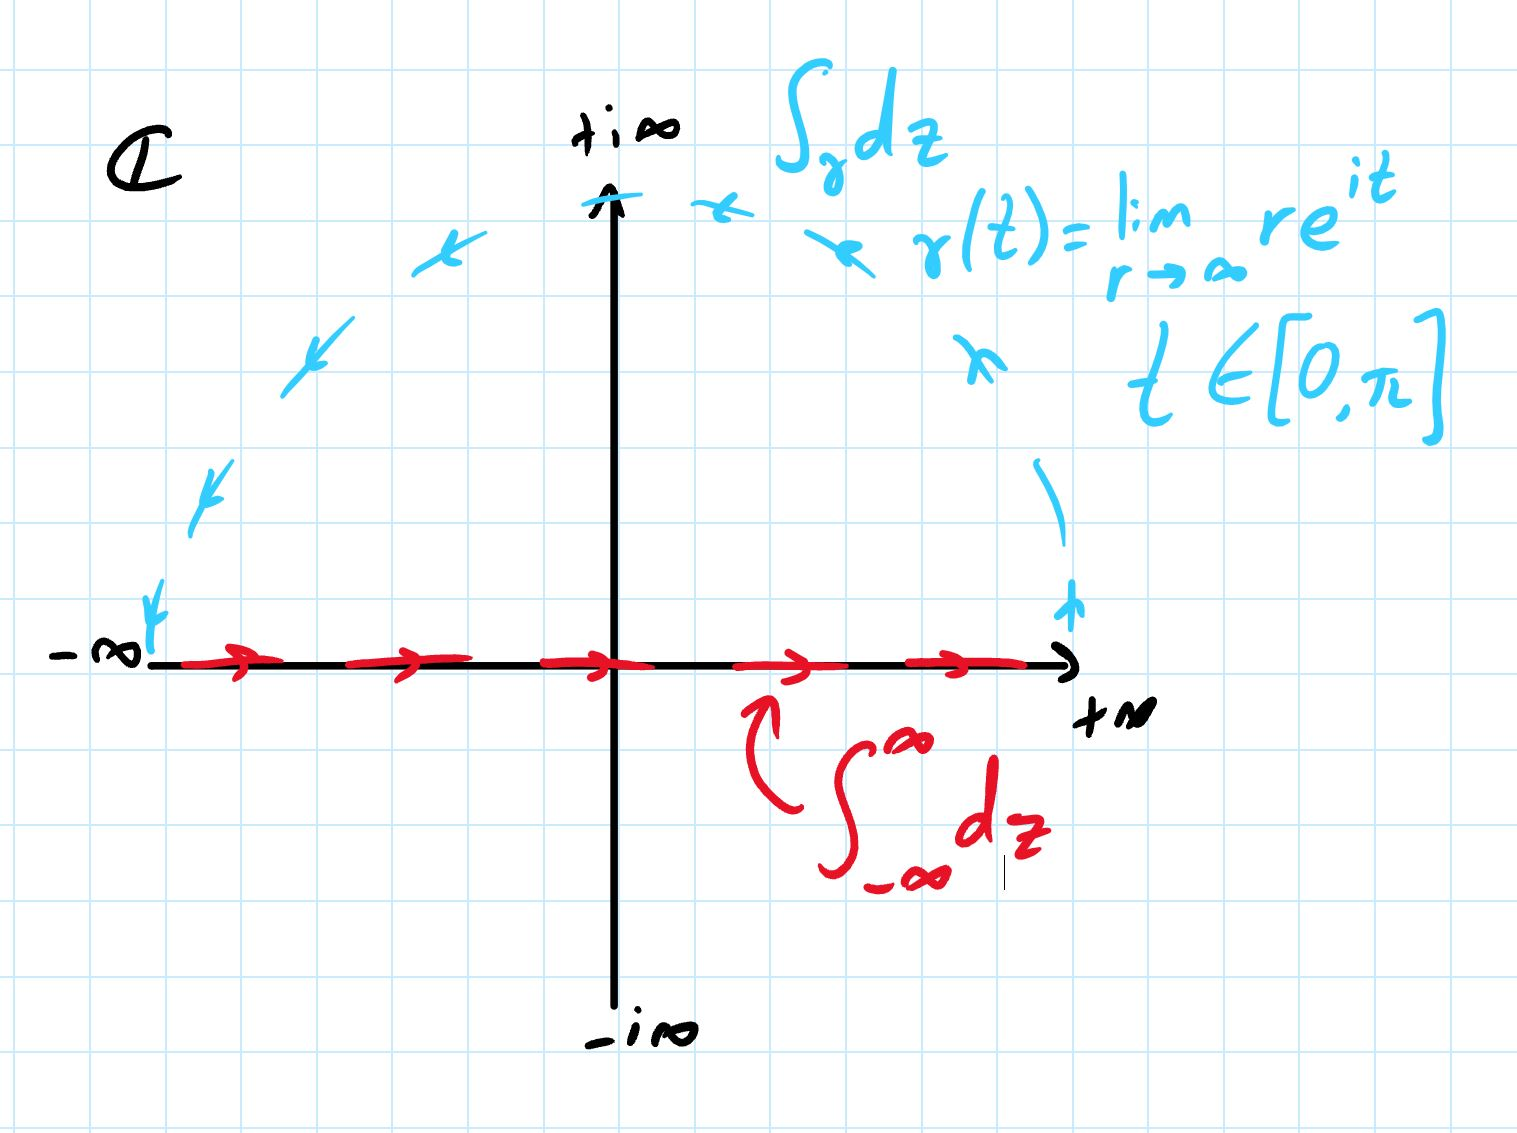
\includegraphics[width=0.8\linewidth]{2018/10/20180704_1.JPG}
\caption{An illustration of closing the contour for a real integral (in red) so we can use the Cauchy integral formula to perform the integral. The integral along the light blue curve $\int_\gamma dz$ contributes nothing to the overall integration, so we can use it to close the contour out at $+i\infty$. Note the curve runs counterclockwise. If it ran clockwise, we would pick up a minus sign.}
\end{figure}

How do we decide whether to close the contour in the upper or lower half-plane? Notice that in the upper half-plane, $z=x+iy$ for $y>0$, so $e^{iz}=e^{i(x+iy)}=e^{-y}e^{ix}$ with $y>0$. Therefore, $e^{iz}$ is exponentially damped in the upper half-plane and contributes basically zero to the overall integral. So we can close the curve ''for free'' and write
$$\Int dz \frac{e^{iz}}{z-z_0}=\oint dz \frac{e^{iz}}{z-z_0}=2\pi i e^{iz_0}$$
if $z_0$ has imaginary part $>0$ (is inside the contour) and $0$ otherwise. Thanks, Cauchy integral formula.

In fact, the formula lends itself to an even better generalization, the \term{Cauchy residue theorem}. It states that $$\oint_C f(z)dz = 2\pi i\cdot \text{sum of the residues of }f(z) \text{ inside } C,$$ where the integral around $C$ is in the counterclockwise direction, and a \term{residue} is basically the value at the function at the pole if it didn't have that pole. Quick example: for the function $f(z)=\frac{z}{(1+z)(3-z)}$, $f(z)$ has a pole at $z=3$. The residue $R(3)$ of $f(z)$ at $z=3$ is simply $R(5)=\frac{z}{1+z}|_{z=3}=\frac{3}{4}.$

So to summarize, close the contour based on what the integrand is doing at $\pm i\infty$. Check which poles are inside your contour, and plug up the singularities one at a time to compute the residues. Sum up the residues, multiply by $2\pi i$, and you've got the value of your integral.

Returning to the problem at hand, we wish to compute the integral
$$\int dk^0 \frac{e^{i k^0 x^0}}{(k^0)^2-(\omega_k^2-i\e)}.$$ We have two poles at $\pm\sqrt{\omega_k^2-i\e}$, which in the $\e\to 0$ limit become $+\omega_k-i\e$ and $-\omega_k+i\e$. Therefore, we rewrite as
$$\Int dk^0 \frac{e^{i k^0 x^0}}{(k_0-(\omega_k-i\e))(k_0-(-\omega_k+i\e))}.$$
Since $e^{ik^0x^0}$ is exponentially damped in the upper half-plane, we close the contour at $+i\infty$, enclosing the pole at $-\omega_k+i\e$ (recall $\omega_k$ is real and $\e$ is positive). Therefore, calculating the residue, this integral comes out to
$$2\pi i \frac{e^{-i\omega_k x^0}}{-2\omega_k}$$
(letting $\e\to 0$) and we conclude that for $x^0>0$,
$$\Delta_F(x)=-i \int \frac{d^3 k}{(2\pi)^3 2\omega_k}e^{-i(\omega_k t- \vec{k}\cdot \vec{x})}.$$
A similar calculation holds for $x^0 < 0$, so we recover our friend the Feynman propagator, which correctly accounts for the sign of $x^0$.